\chapter{Progress}

Budd's sliding theory describes stress propagation through flowing ice over undulating bedrock. The stress field propagates upward at an angle, creating surface (elevation) waves that are phase-shifted by approximately $\pi/2$ relative to bedrock (elevation) features, in Budd's words: \texttt{\texttt{the maximum shear stress occurs at the tops of the waves and the minimum in the troughs''\cite{Budd_1970}}}. 

----WHAT GOES HEREEEEE---- 
% provides insight into ice stress transmission and response times.---

My work up until now has been focused in building a comprehensive computational framework developed for the systematic investigation of ice dynamics. The first part of this framework is to study via simulations in 2D the ice flowline behavior over a variety of synthetic bedrock topographies to understand the relationship between basal geometry, ice rheology, and overall flow response. A key aim of this work is to understand the effect of commonly made assumptions in ice sheet modelling and their repercussions in the validity of resulting models. This initial stage is designed to be a complete, end-to-end pipeline, from environment setup to final scientific analysis. 

\section{The Computational Framework of this Study}

This study is supported by a suite of interconnected scripts and tools designed for generating conditions, running simulations, processing output, and performing scientific analysis.

\subsection{Synthetic Bedrock Generation}

The \texttt{bedrock\_generator.py} script generates synthetic 1D bedrock profiles for ice flow modeling. the core functionality of this script is the creation of realistic bedrock topographies with configurable geometric properties. The bedrock profiles are defined by the following four key parameters that can be varied systematically:
\begin{itemize}
\item{Amplitude} Controls the vertical scale of undulations (e.g., 19.2 m to 38.4 m).
\item{Wavelength} Controls the horizontal scale of undulations (e.g., 3.84 km to 19.2 km).
\item{Skewness} Controls the asymmetry of the undulations.
\item{Kurtosis} Controls the peakedness or flatness of the features.
\end{itemize}

The generated profiles are saved to \texttt{.npz} files and are loaded by the ice flow simulation script to ensure consistent and reproducible experimental setups.

\subsection{Ice Flow Simulation}

The core of the project is an ice flow modeling script (\texttt{flowline.py}) built upon the Ice-sheet and Sea-level System Model (ISSM). The simulation solves the full-Stokes ice flow equations for a static diagnostic stress balance setup and a transient run (this includes stress balance and mass transport configurations). The simulation utilises the Bidimensional Anisotropic Mesh Generator (BAMG) for the case of 2D flowband meshes (\texttt{bamgflowband}) to create meshes where the mesh resolution is refined based on the underlying bedrock wavelength to capture key physics efficiently.

The experimental design is built around four benchmark experiments to test different physical conditions:

\begin{enumerate}
\item{S1} No-slip (frozen) bed + Linear rheology ($n=1$).
\item{S2} No-slip (frozen) bed + Non-linear rheology ($n=3$).
\item{S3} Linear sliding + Linear rheology ($n=1$).
\item{S4} Linear sliding + Non-linear rheology ($n=3$).
\end{enumerate}

The \texttt{flowline.py} script produces \texttt{.nc} files and binary \texttt{.outbin} files for full simulation results (when run locally and on the NCI Gadi system respectively). The \texttt{flowline.py} script can also generate text files for quick analysis in the case of the static diagnostic runs.

\subsection{Data Processing and Visualization Tools}

A series of robust, high-performance scripts were developed to handle the large volume of data produced by the simulations. (Note that: All these scripts have individual file processing capabilities)

\begin{enumerate}
\item{Binary to NetCDF Conversion} A batch-capable tool (\texttt{batch\_convert.py}) converts ISSM's proprietary \texttt{.outbin} files into the standard, portable NetCDF format. This script supports parallel processing for high throughput.
\item{Result Extraction and Visualization} A batch script (\texttt{batch\_extract\_results.py}) that automatically finds and processes NetCDF files to generate visualisations of key fields like velocity and pressure. 
\item{Targeted Scientific Plotting} Additional scripts (\texttt{batch\_plots.py}) are used to create specific scientific plots, such as basal velocity oscillations colored over the bed topography and basal shear stress distributions, to analyse the direct impact of the bedrock on flow.
\end{enumerate}

\subsection{Scientific Analysis Tools}

In order to  perform quantitative analysis on the simulation results. I developed a pair of Grid Convergence Analysis scripts capable of analysing the resolution convergence in both the static and transient runs \texttt{analyse\_grid\_convergence.py} and \texttt{analyse\_transient\_convergence.py} respectively. Convergence is assessed by comparing solutions from different mesh resolutions (e.g., factors of 0.5, 0.75, 1.0, 1.5) against the finest mesh solution. The primary metric of this script is the L2 relative error, a global, scale-independent measure that quantifies the overall difference between two solutions. An error below $1\%$ is typically considered a sign of good convergence. A standardized $2\times2$ plot is generated to provide a comprehensive view of convergence, showing visual velocity comparisons, numerical L2 error bars, and the computational cost of each resolution.

To quantify the spatial phase shift between the bedrock topography and the ice surface response and verify the physical validity of my simulation based on the criteria in \cite{Budd_1970}, 
I developed a single and a batch-processing scripts (\texttt{phase\_analysis.py} and \texttt{batch\_phase\_analysis.py}) that use cross-correlation to calculate the lag and phase shift between the de-trended bed and surface signals for each time step in a given simulation. The scripts generates time-series plots of phase shift evolution and summary text files with numerical results. For each batch or single simulations analysed.

\subsection{Key Findings: The Grid Independence and Stability Study}

In order to validate my simulation outputs, I performed grid independence study to determine the optimal mesh resolution that balances computational cost and numerical accuracy. This study led me to a critical discovery that reshaped my simulation strategy.

My diagnostic convergence analyses yielded realistic results and showed that, for a single test profile (022 in Experiment S4), coarser resolutions appeared to provide marginally adequate accuracy when compared to the finest resolution factor $0.5$ of the original element size generated by 

\begin{table}[h]
\centering
\caption{Corrected Diagnostic Convergence for Profile 022 (Experiment S4)}
\begin{tabular}{llll}
\toprule
Resolution & Surface vx L2 Error & Basal vx L2 Error & Convergence Status \\
\midrule
0.75 & 0.41\% & 0.22\% & \textbf{EXCELLENT} \\
1.0 & 0.34\% & 1.30\% & \textbf{MARGINAL} \\
1.5 & 1.17\% & 1.18\% & \textbf{INADEQUATE} \\
\bottomrule
\end{tabular}
\end{table}

\subsubsection{Critical Discovery: The Transient Stability Crisis}

Based on the promising diagnostic results, I launched a wider study using multiple bedrock profiles. This revealed a dramatic and critical disconnect between diagnostic accuracy and transient simulation stability. While coarser meshes showed acceptable *diagnostic* error, they consistently failed during *transient* simulations.

\begin{table}[h]
\centering
\caption{Transient Simulation Stability Across 5 Distinct Profiles (Experiment S4)}
\begin{tabular}{llll}
\toprule
Resolution & Profiles Completed & Success Rate & Stability Status \\
\midrule
0.5 & 5/5\% & 100\% & \textbf{STABLE} \\
0.75 & 2/5\% & 40\% & \textbf{UNSTABLE} \\
1.0 & 1/5\% & 20\% & \textbf{VERY UNSTABLE} \\
1.5 & 0/5\% & 0\% & \textbf{CRITICAL FAILURE} \\
\bottomrule
\end{tabular}
\end{table}
The profiles summarised here are 027, 164, 285, 433, 692. All these profiles represent different combinations of amplitudes, wavelength, skewness and kurtosis values. These findings demonstrates that good diagnostic convergence does not guarantee transient stability. Further analysis showed that stability is highly dependent on the specific bedrock geometry, with some profiles being far more sensitive to coarse resolution than others, The profiles that appear to be the most problematic are those with a parameter combination of high amplitude and short wavelength.

\subsubsection{Opting for a``Stability-First'' Strategy}

This stability crisis prompted a fundamental shift in the project's methodology, away from balancing accuracy and efficiency, and towards prioritizing simulation reliability. These findings lead me to define the production standard resolution factor of $0.5\times$ standard element size generated by \texttt{bamgflowband} as the only production-viable choice for transient simulations.

\section{RESULTS}

% \begin{figure}[H]
%     \includegraphics[scale=0.5]{basal\_friction.png}
%     \caption{Slope parallel visualisation of the computational mesh with basal nodes highlighted. The gray dotted lines represent the complete finite element mesh with multiple vertical layers conforming to the undulating geometry. Basal nodes (purple to yellow) follow the periodic undulated bed topography with wavelength 9.72 km and amplitude 0.054 km. The colour gradient along the basal nodes displays the imposed variations in basal shear stress corresponding to Budd's sliding law, with lighter colours indicating regions of higher basal drag. Note that maximum basal drag occurs near the peaks of the bedrock undulations, consistent with the expected shear stress pattern in the sliding theory. The 27 km domain contains approximately three complete undulation cycles.}
%     \label{fig:friction}
% \end{figure}

% \begin{figure}
%     \includegraphics[scale=0.45]{Pressure\_300yrs\_xz.png}
%     \caption{Pressure field distribution at t = 300.00 years shown in original coordinates. The color scale reveals the spatial pressure variations throughout the ice body, with higher pressures (yellow) concentrated at the base and particularly near bedrock peaks. The triangular mesh elements display the finite element discretisation used for solving the Full-Stokes equations. The overall pressure gradient follows ice thickness with maximum values at the base with a visible influence of bedrock undulations on the pressure field. The downward-sloping ice surface reflects the -0.1 radian background slope condition, while subtle surface undulations are apparent in response to the bed topography. This visualization captures the result after 300 years of transient simulation, providing insight into the stress propagation patterns described in Budd's sliding theory.}
%     \label{fig:Pressure}
% \end{figure}
% % Note: The white gaps visible within the mesh represent masked areas excluded from visualization processing, not physical features or data gaps in the original simulation.

% \begin{figure}
%     \includegraphics[scale=0.45]{Vx\_300yrs\_xz.png}
%     \caption{
%     Horizontal velocity field ($V\_x$) at t = 300.00 years displayed in original coordinates. The color scale indicates velocity magnitudes ranging from 0 to 0.0147 km per year with flow direction from left to right. The velocity pattern shows clear acceleration as the ice flows downslope, with highest velocities (yellow) occurring near the terminus region. The fixed upstream boundary condition constrains flow at the inlet, while the progressive acceleration downstream results from gravitational forcing along the -0.1 radian sloped bed. Note the visible influence of the bedrock undulations on the velocity field, particularly near the base. The contrast between slow-moving upper ice (purple) and faster basal ice in the terminal region demonstrates the development of vertical velocity gradients.}
%     \label{fig:Vx}
% \end{figure}


% \begin{figure}
%     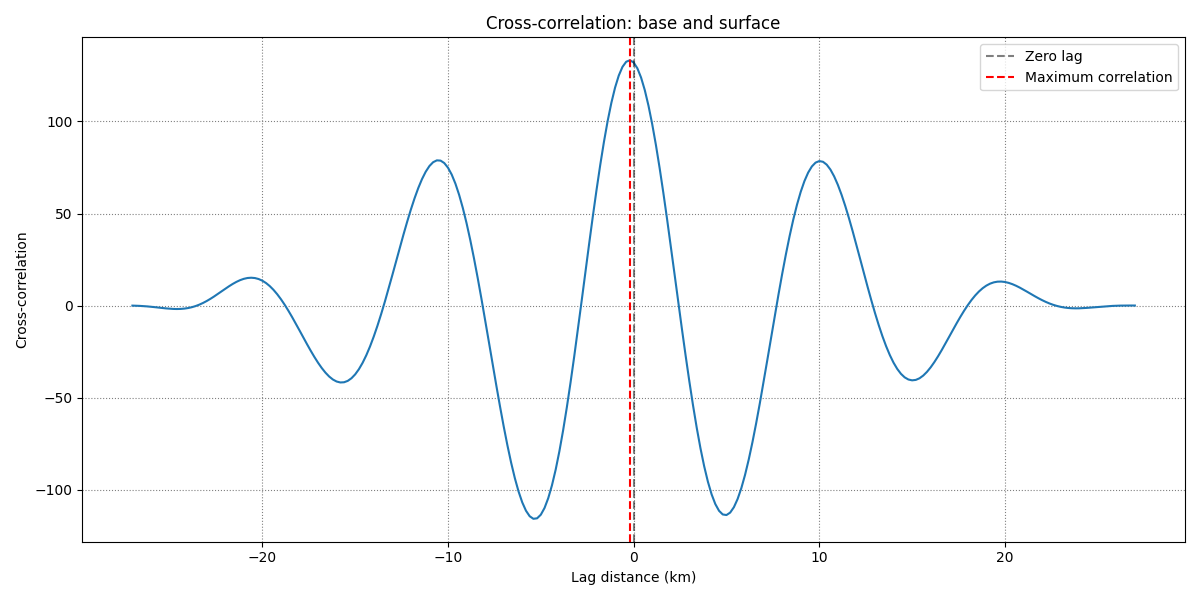
\includegraphics[scale=0.5]{xcorr.png}
%     \caption{Cross-correlation between the bedrock elevation and surface slope signals across spatial lags. The blue curve shows normalized correlation coefficients as a function of lag distance. The maximum correlation (red dashed line) occurs at a lag distance of -0.2 km, which translates to a phase shift of -0.04$\pi$ radians (-7.4 degrees). This observed phase shift significantly deviates from Budd's theoretical prediction of $\pi/2$ (90 degrees), suggesting that in this simulation at t = 300 years, the relationship between bedrock topography and surface features differs from theory. The zero lag position (black dashed line) represents perfect spatial alignment. The periodic nature of the cross-correlation function reflects the underlying 9.72 km wavelength of the bedrock undulations, with correlation peaks appearing at approximately 10 km intervals.}
%     \label{fig:xcorr}
% \end{figure}

% \begin{figure}
%     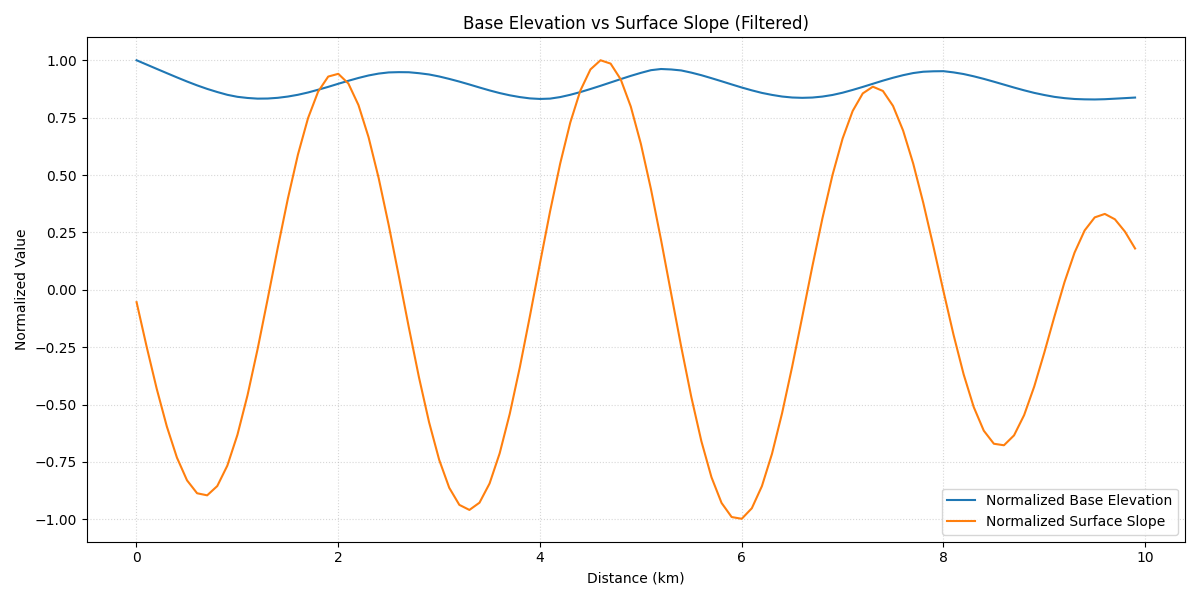
\includegraphics[scale=0.5]{direct.png}
%     \caption{Direct comparison between bedrock topography (black) and ice surface elevation (blue) with mean elevations removed to highlight the undulation patterns. Both profiles are plotted in slope-parallel coordinates along the 27 km domain. The surface undulations exhibit a visible phase shift relative to the bedrock features, though this shift is noticeably less than the theoretical $\pi/2$ predicted by Budd's sliding theory. The surface amplitude appears damped compared to the bed amplitude, particularly evident in the central wavelengths. However, boundary effects near $x = 0$ and $x = 27$ km complicate the interpretation, as the amplitude damping and phase relationships may be influenced by the finite domain and boundary conditions. This comparison at t = 300 years reveals a complex and still-evolving relationship between bed topography and surface expression, with the phase relationship varying slightly across the domain. The dominant wavelength of approximately 9.72 km is preserved in both signals, indicating effective stress transmission through the 2.7 km ice thickness despite the reduced phase shift.}
%     \label{fig:direct}
% \end{figure}

% \begin{figure}
%     \includegraphics[scale=0.45]{surfaces\_comparison.png}
%     \caption{Evolution of ice surface topography from initial condition (black) to final state at t = 300.00 years (red) displayed in original coordinates. The simulation shows significant ice thinning and terminus retreat, with the final surface elevation ranging from -0.57 to 3.73 km compared to the initial range of 1.00 to 3.74 km. The final surface exhibits a steeper overall slope, particularly in the lower half of the domain ($x > 15$ km), indicating a dynamic response to the applied flow conditions. Surface undulations have developed in the final state, though these are subtle relative to the overall elevation change. The preservation of similar elevation at the upper boundary ($x = 0$ km) reflects the fixed inflow boundary condition, while the downstream region shows maximum adjustment. This 300-year evolution demonstrates that the ice mass is still adapting to the prescribed basal conditions and has not yet reached a steady state, which may explain the discrepancy between the observed phase shift and Budd's theoretical prediction.}
%     \label{fig:surfaces}
% \end{figure}

